\documentclass[11pt]{article}
\usepackage{geometry}                % See geometry.pdf to learn the layout options. There are lots.
%\geometry{letterpaper}                   % ... or a4paper or a5paper or ...
%\geometry{landscape}                % Activate for for rotated page geometry
%\usepackage[parfill]{parskip}    % Activate to begin paragraphs with an empty line rather than an indent
\usepackage{graphicx}
\usepackage{amsmath}
\usepackage{amssymb}
\usepackage{epstopdf}
\usepackage{mathtools}
\DeclareGraphicsRule{.tif}{png}{.png}{`convert #1 `dirname #1`/`basename #1 .tif`.png}

\newcommand{\bbR}{\mathbb{R}}
\newcommand{\bbZ}{\mathbb{Z}}
\newcommand{\vb}{\vec{b}}
\newcommand{\vv}{\vec{v}}
\newcommand{\vvs}{\vec{v}^*}
\newcommand{\vbs}{\vec{b}^*}
\newcommand{\sspan}{\mathsf{span}}
\newcommand{\vol}{\mathrm{vol}}
\newcommand{\GH}{\mathrm{GH}}
\newcommand{\ENUMCost}{\mathrm{ENUMCost}}
\newcommand{\MINCost}{\mathrm{MINCost}}
\newcommand{\SimENUMCost}{\mathrm{Sim}\text{-}\mathrm{ENUMCost}}
\newcommand{\Costbeta}{\mathrm{Cost}_{\beta}}
\newcommand{\SimGSLengths}{\mathrm{Sim}\text{-}\mathrm{GS}\text{-}\mathrm{Lengths}}
\newcommand{\SimFEC}{\mathrm{Sim}\text{-}\mathrm{FEC}}
\newcommand{\SimGH}{\mathrm{Sim}\text{-}\mathrm{GH}}
\newcommand{\TimeBKZ}{\mathrm{TimeBKZ}}

\title{BKZ Algorithms: An Introduction}
\author{Yuncong Zhang}
%\date{}                                           % Activate to display a given date or no date

\begin{document}
\maketitle

\section{Introduction}

The \emph{Shortest Vector Problem} (SVP) is finding the shortest non-zero vector in a lattice $L$ given the basis $(\vb_1,\cdots,\vb_n)$.
The norm of the shortest non-zero vector in $L$ is denoted by $\lambda_1(L)$.
The approximation version of SVP is denoted by $\gamma$-SVP, which is finding a vector in $L$ whose norm is at most $\gamma(n)\lambda_1(L)$.
Obviously, $\gamma(n)\geq 1$ is necessary for a meaningful $\gamma$-SVP problem, since by definition it is impossible to find a vector with norm less than $\lambda_1(L)$.
For $\gamma=1$, the $\gamma$-SVP is the original SVP.
The quality of SVP solving algorithms are measured by $\gamma$, i.e. the smallest $\gamma$ such that they can solve $\gamma$-SVP.

The current algorithms to solve SVP can be categorized into three classes.
One class is the blockwise algorithms, which usually optimize the basis as a whole.
Given appropriate parameters, these algorithms typically solves the SVP problem in polynomial time, with the approximation factor being exponential.
The blockwise algorithms starts with the famous LLL reduction, and the ones that currently perform the best are the BKZ algorithms.
The original BKZ algorithm was proposed by C. P. Schnorr \cite{se1994lattice} in 1994.
It was then improved in various aspects, and such improvements were gathered into a new version of BKZ called BKZ 2.0 \cite{cn2011bkz}. Specifically, the improvements adopted in BKZ 2.0 include extreme pruning in enumeration, early termination, local-block preprocessing, and limiting the point searching in enumeration by Gaussian Huristic.

Progressive BKZ is a type of BKZ algorithms that implement the strategy of adaptively increasing the blocksize.
However, it is challenging to find an optimal strategy to increase the blocksize so that the computational cost is minimized.
BKZ 2.0 uses a progressive BKZ in the local-block preprocessing in each step, though it does not use it globally.

Blockwise algorithms such as BKZ works together with another category of SVP solving algorithm called the enumeration algorithm.
The enumeration algorithm, contrary to the blockwise algorithms, is able to find the exact solution to SVP, but requires expoenential time w.r.t. the lattice dimension.
The blockwise algorithms and enumeration algorithms rely heavily on each other.
In fact, BKZ repeatedly invokes enumeration algorithm to solve SVP in the local block which is a lattice of small dimension.
On the other hand, the efficiency of enumeration algorithms is significantly impacted by the quality of the input basis.
Therefore, the enumeration algorithms usually require the input to be preprocessed by a blockwise algorithm.

The last category of algorithms solving SVP is called \emph{sieving}.
This kind of algorithms require large amount of memory, and was considered insignificant compared to blockwise and enumeration algorithms \cite{gnr2010lattice}.
However, the sieving algorithms have been developing rapidly recently, and is currently occupying the first positions in the TU Darmstadt Lattice Challenge.
However, these algorithms are not much relevant to the topic in this article, so we will not cover them in the following.

This article aims to provide an illustration of the state-of-the-art BKZ algorithms.
We start with necessary preliminaries to understand BKZ in Sec. \ref{sec:pre}.
Sec. \ref{sec:basic} describes the most basic BKZ algorithm.
The improvements by BKZ 2.0 is explained in Sec. \ref{sec:bkz2}.
Sec. \ref{sec:pbkz} and Sec. \ref{sec:ipbkz} give the progressive BKZ algorithms.
Finally, Sec. \ref{sec:con} concludes this article.

\section{Preliminaries}
\label{sec:pre}

\subsection{Gram-Schmidt Basis}

Given a lattice $L=L(\vb_1,\cdots,\vb_n)=\left\{\sum x_i\vb_i:x_i\in\bbZ\right\}$ of dimension $n$, and its basis $B=(\vb_1,\cdots,\vb_n)$, the Gram-Schmidt reduction of the basis $B$ is defined as $B^*=(\vb_1^*,\cdots,\vb_n^*)$, where $\vb_i^*=\vb_i-\sum_{j=1}^{i-1}\langle\vb_i,\vb_j^*\rangle\vb_j^*/\|\vb_j^*\|^2$.
For simplicity, let $\mu_{ij}=\langle\vb_i,\vb_j^*\rangle/\|\vb_j^*\|^2$ and call it the \emph{Gram-Schmidt coefficient} of $B$.
Similarly, $\|\vb_j^*\|$ is called the \emph{Gram-Schmidt lengths}.
Notice that $B^*$ is not necessarily a basis for lattice $L$, since the Gram-Schmidt coefficients are not restricted to be integers, though it is still a basis of the linear space spanned by $B$.
The Gram-Schmidt reduced basis $B^*$ is an orthogonal basis for the linear space $\sspan(\vb_1,\cdots,\vb_n)$.
Moreover, each $\vb_i^*$ is perpendicular to the space $\sspan(\vb_1,\cdots,\vb_{i-1})=\sspan(\vb_1^*,\cdots,\vb_{i-1}^*)$.

The Gram-Schmidt reduction does not change the determinant of the basis $\det(L):=\det(\vb_1,\cdots,\vb_n)$.
To see that, notice that in each step of the reduction, the difference between $\vb_i^*$ and $\vb_i$ is a vector $\vb_i-\vb_i^* \in \sspan(vb_1,\cdots,\vb_{i-1})$.
Since $\det(\vb_1,\cdots,\vb_n)$ is linear w.r.t each vector, we have
\begin{eqnarray}
\det(\vb_1,\cdots,\vb_i,\cdots,\vb_n)=\det(\vb_1,\cdots,\vb_i-\vb_i^*,\cdots,\vb_n)+\det(\vb_1,\cdots,\vb_i^*,\cdots,\vb_n) \label{eqn:det-sum}
\end{eqnarray}

The first summand of (\ref{eqn:det-sum}) is $0$, since $\vb_i-\vb_i^*$ is not linearly independent from $(\vb_1,\cdots,\vb_{i-1})$.
Therefore, we conclude that each step of the Gram-Schmidt reduction does not affect the determinant.
This conclusion applies to the entire reduction, i.e. $\det(B^*)=\det(B)$.

Since $B^*$ is an orthogonal basis, we also have $\det(B^*)=\prod_{i=1}^n \|\vb_i^*\|$.
This is the volume of the $n$-dimensional rectangle spanned by the vectors in $B^*$.
In fact, this is also the volume of the $n$-dimensional \emph{parallelepiped}, namely a cell of the lattice, spanned by the vectors in $B$.
Therefore, we also use the notation $\vol(L):=\det(L):=\det(B)$ interchangably.

\begin{figure}[ht!]
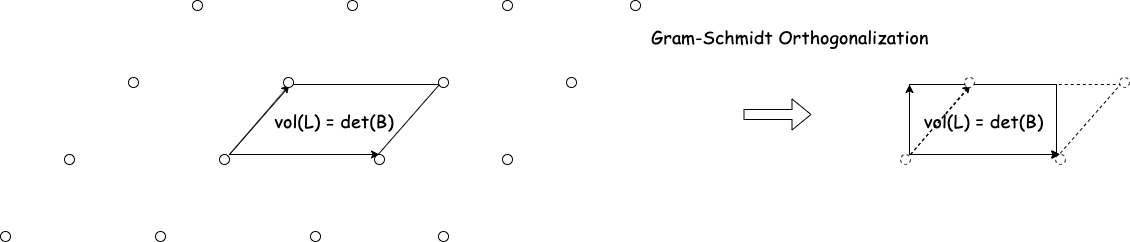
\includegraphics[width=0.8\textwidth]{files/BKZ-Volume.png}
\caption{Gram-Schmidt orthogonalization and volume of lattice}
\label{fig:bkz.volume}
\end{figure}

Fig.\ref{fig:bkz.volume} illustrates how Gram-Schmidt orthogonalization transforms a parallelepiped into rectangle, and the fact that the transformation does not change the volume of the basis.
Note that the Gram-Schmidt reduced basis $B^*$ is no longer a basis of the original lattice.
However, it is frequently used in the analysis of the efficiency of the SVP algorithms.

\paragraph{Geometric Series Assumption (GSA).} The GSA introduced by Schnorr says that the Gram-Schmidt reduced basis vectors decreases by a constant $r$ with the increment of $i$.
Specifically, $\|\vb_i^*\|^2/\|\vb_1\|^2=r^{i-1}$, where $r\in[3/4,1)$ is called the GSA constant.


\subsection{Projective Sublattice}

We define the projection $\pi_i:\bbR^n\to\sspan(\vb_1,\cdots,\vb_{i-1})^{\perp}$ as in equation (\ref{eqn:pi}):

\begin{eqnarray}
\pi_i(v):=\vec{v}-\sum_{j=1}^{i-1}\langle\vec{v},\vb_j^*\rangle\vb_j^*/\|\vb_j^*\| \label{eqn:pi}
\end{eqnarray}

Obviously, this is the same as the definition of one step in the Gram-Schmidt reduction.
With this notion, the Gram-Schmidt reduction can be expressed as follows: for $i$ from $1$ up to $n$, $\vb_i^* = \pi_i(\vb_i)$.
In fact, this projection removes the proportion of the vector inside the space $\sspan(\vb_1,\cdots,\vb_{i-1})$, and leaves the part that is in $\sspan(\vb_1,\cdots,\vb_{i-1})^{\perp}$.
In particular, $\pi_1(\cdot)$ is the identity map, and for $i>0$, $\pi_i(\cdot)$ projects the entire space $\sspan(\vb_1,\cdots,\vb_{i-1})$ to zero, including all the basis, i.e. $\vb_{j}$ for $1\leq j<i$.

We further define the \emph{local-block} of size $\beta=j-i+1$ as the projective sublattice:

\begin{eqnarray}
L_{[i:j]} &:=& \pi_i(L(\vb_i,\vb_{i+1},\cdots,\vb_j)) \nonumber \\
&:=&L(\pi_i(\vb_i),\pi_i(\vb_{i+1}),\cdots,\pi_i(\vb_{j}))
\end{eqnarray}

This is the lattice obtained by projecting all the vectors in $L(\vb_i,\vb_{i+1},\cdots,\vb_j)$ by $\pi_i$.
The second equality can be easily deduced from linearity of $\pi_i$.

In fact, since $\pi_i$ zerofy the entire subspace $\sspan(\vb_1,\cdots,\vb_{i-1})$, it is equivalent to define $L_{[i:j]}$ as $\pi_i(L(\vb_1,\cdots,\vb_{j}))$.

Fig.\ref{fig:proj} illustrates how a projection works on lattice in the simple $2$-dimensional case.

\begin{figure}[ht!]
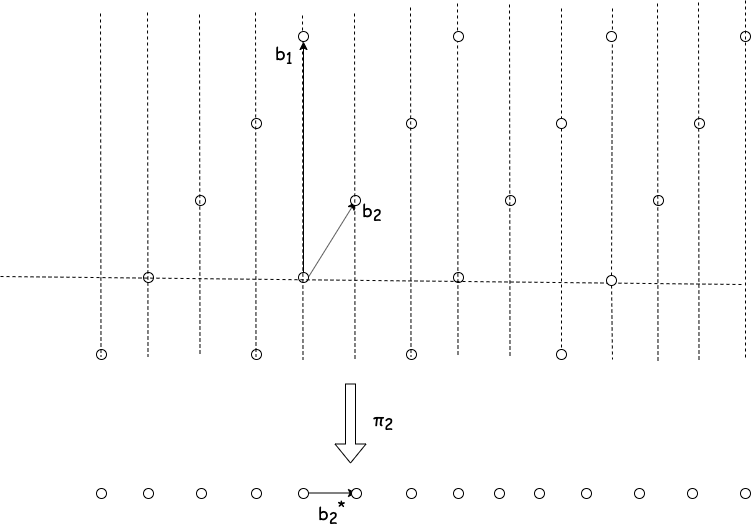
\includegraphics[width=0.8\textwidth]{files/BKZ-Projection.png}
\caption{Projection $\pi_2$ on a lattice}
\label{fig:proj}
\end{figure}

For simplicity, we use the notation $B_i$ for the local-block lattice $L_{[i:j]}$ when the blocksize $\beta$ (thus the value of $j$) is clear in the context.

\subsection{Gaussian Huristic}

The \emph{Gaussian Huristic} is an estimation of the number of lattice points contained in an $n$-dimensional convex set $S$.
It basically says that the number of lattice points contained in the set, denoted by $|S\cap L|$, is approximately proportional to the volume of the set.
As we can image, the lattice points spread very evenly over the entire $\bbR^n$ space, it is not hard to understand this huristic.
Specifically, the Gaussian Huristic says that $|S\cap L|\approx\vol(S)/\vol(L)$.
Recall that $\vol(L)$ is the volume of the parallelepiped spanned by a basis of $L$, i.e. a cell of the lattice.
This is also understandable, since the number of cells contained in $S$ is approximately the number of lattice points contained in $S$.

Fig.\ref{fig:gh} is an example where a $2$-dimensional ball (i.e. a circle) contains $6$ lattice points.
The size of the ball is roughly $6$ times of the size of a lattice cell.

\begin{figure}[ht!]
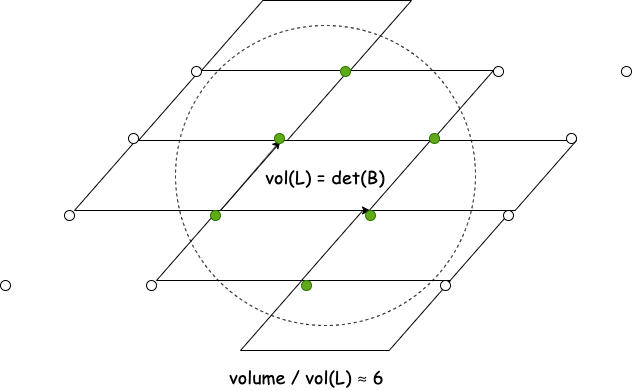
\includegraphics[width=0.8\textwidth]{files/BKZ-Gaussian-Huristic.png}
\caption{Gaussian Huristic for $2$-dimensional Lattice}
\label{fig:gh}
\end{figure}

The convex shape that we care most about is $n$-dimensional ball.
Denote by $V_n(R)$ the volume of an $n$-dimensional ball with radius $R$.
We have the following equation:
\begin{eqnarray}
V_n(R) = R^n\cdot\frac{\pi^{n/2}}{\Gamma(n/2+1)}
\end{eqnarray}
where $\Gamma(x)$ is the gamma function, which is defined by $\Gamma(x)=\int_0^{\infty}t^{s-1}\cdot e^{-1}dt$.

The Gaussian heuristic of the shortest vector of $L$, i.e. $\lambda_1(L)$, is the radius of the ball with the same volume as a cell of the lattice.
That is the solution of $V_n(x)=\vol(L)$, which is:

\begin{eqnarray}
(\vol(L)/V_n(1))^{1/n} = \left(\frac{\Gamma(n/2+1)\vol(L)}{\pi^{n/2}}\right)^{1/n}=\frac{(\Gamma(n/2+1)\vol(L))^{1/n}}{\pi^{1/2}}
\end{eqnarray}

This is denoted by $\GH(L)$, which is often used as a ``prediction'' of $\lambda_1(L)$.
There are also counterexamples to this heuristic.

The Hermite constant $\gamma_n$ is the supreme of $(\lambda_1(L)/\vol(L)^{1/n})^2$ over all lattices.
By Minkowski's theorem, $\sqrt{\gamma_n}\leq 2\cdot V_n(1)^{-1/n}$.
From this we obtain that $\lambda_1(L)\leq 2\GH(L)$.

\paragraph{Gaussian Heuristic for Projective Lattices.} The length $\lambda_1(B_i)$ of the shortest vector in the projective local lattice for small blocksizes $\beta$ \cite{cn2011bkz}.
Recall that a projective local lattice $B_i$ is the lattice $\pi_i(L(\vb_i,\cdots,\vb_{i+\beta-1}))$.
Denote the ratio between $\lambda_1(B_i)$ and $\GH(B_i)$ for block of dimension $\beta$ by $\tau_{\beta}$, and call it the coefficient of modified Gaussian heurstic.
According to the simulation provided in \cite{cn2011bkz}, $\tau_{\beta}$ decreases with $\beta$, and for $\beta>50$, $\tau_{\beta}$ is very close to $1$, i.e. $\lambda_1(B_i)$ is close to $\GH(B_i)$ for large values of $\beta$.
Therefore, it is reasonable to estimate $\lambda_1(B_i)=\tau_i\GH(B_i)$ for $\beta\leq 50$, and $\lambda_1(B_i)=\GH(B_i)$ for $\beta>50$.

\subsection{Enumeration Algorithm}

The enumeration algorithm \cite{gnr2010lattice} searches for the shortest vector in a lattice.
Given a lattice basis $B=(\vb_1,\cdots,\vb_n)$, the shortest vector $\vvs$, like any vectors in the lattice, can be expressed as a combination of the basis with integer coefficients.
Let

\begin{eqnarray}
\vvs=a_1\vb_1+a_2\vb_2+\cdots+a_n\vb_n\qquad\forall i\in[n]
\end{eqnarray}

Finding the shortest vector is equivalent to determining the coefficients $a_i$ for all $i\in[n]$.
However, the values of each of the $a_i$ is boundless, which renders naive searching extremely impractical.

The enumeration algorithm exploits the following fact: for each $i\in[n]$, $\|\pi_i(\vvs)\|\leq\|\vvs\|$, since $\pi_i(\vvs)$ is a projection of $\vvs$ onto a subspace of $\bbR^n$.
Therefore, by the fact that $\pi_i(\cdot)$ vanishes on $\sspan(\vb_1,\cdots,\vb_{i-1})$, we have
\begin{eqnarray}
\|\pi_i(a_i\vb_i+\cdots+a_n\vb_n)\|=\|\pi_i(\vvs)\|\leq\|\vvs\|\qquad\forall i\in[n] \label{eqn:enum-bound}
\end{eqnarray}

Equation (\ref{eqn:enum-bound}) gives us a bound for the coefficients.
Starting from $k=n$, we have $\|\pi_n(a_n\vb_n)\|=\|a_n\pi_n(\vb_n)\|\leq\|\vvs\|$, which limits the values of $a_n$ to a set of finite size.
Fixing $a_n$ to each candidate, the value of $a_{n-1}$ is also restricted to a finite set.
Continuing this procedure, for each selection of $(a_k, a_{k+1}, \cdots, a_n)$, $a_{k-1}$ is restricted to a finite set of values.

Therefore, the entire set of possible combinations of $(a_1,\cdots,a_n)$, that is, all the possible vectors $\vv$, forms a tree.
At the root of the tree is the zero vector.
The first layer of the tree consists of all the vectors $a_n\vb_n$ such that $\|a_n\pi_n(\vb_n)\|\leq\|\vvs\|$.
For each vector $\vv$ in the $k$'th layer of the tree, its children consists of all the vectors $\vv+a_{n-k}\vb_{n-k}$ such that $\|\vv+a_{n-k}\pi_{n-k}(\vb_{n-k})\|\leq\|\vvs\|$.
Fig.\ref{fig:search-tree} shows the structure of the searching tree, and gives an example of the vertices in a $2$-dimensional searching tree.

\begin{figure}[ht!]
	\centering
	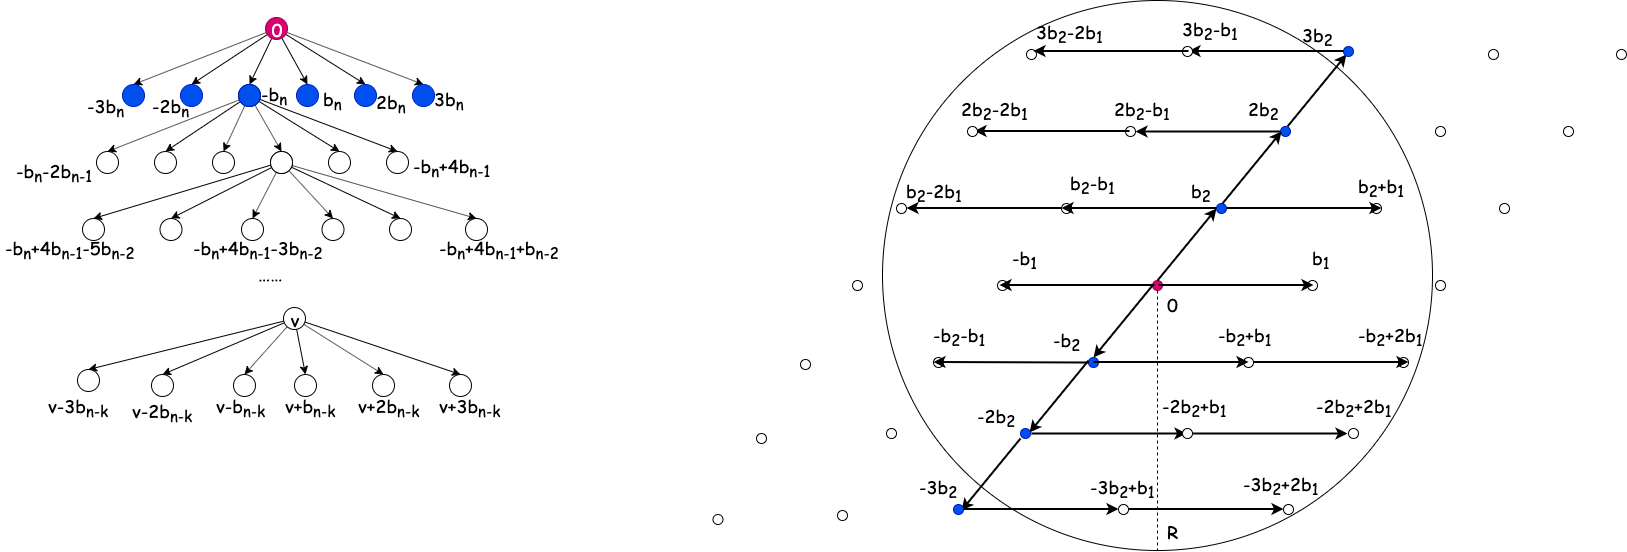
\includegraphics[width=0.8\textwidth]{files/BKZ-Searching-Tree.png}
	\caption{Searching Tree}
	\label{fig:search-tree}
\end{figure}

However, we have no idea what $\|\vvs\|$ is before we actually find $\vvs$.
Therefore, we must replace this bound with some value $R$ that we already know.
Of course, if we choose $R$ to be larger than $\|\vvs\|$, such as $\|\vb_i\|$ for any $i$, this algorithm will successfully find $\vvs$ with probability $1$, but the amount of computation increases for larger $R$.
On the other hand, smaller $R$ improves the efficiency, but decreases the success probability.
Further more, for different layers, we can use a seperate bound $R_k$.
Selecting these bounds is a major point of research for improvement of the enumeration algorithm.

The computational cost of the enumeration algorithm is measured by the number of nodes in the searching tree, which is denoted by $N$.
Chen-Nguyen found a method to minimize $N$ subject to a probability $p$ to successfully find a vector of length less than $\alpha\cdot\GH(L)$, where $\alpha >0$ is a parameter.
We use $\ENUMCost(B;\alpha,p)$ to denote the computational cost $N$ to find a short vector in $B$ under these parameters.

\subsection{LLL Algorithm}

LLL is used as a subprocedure of the basic BKZ algorithm.
The name is an acronym of its authors, A.K. Lenstra, Jr Lenstra, and L. Lovasz.
It is possible to understand BKZ while regarding LLL as a blackbox.
In fact, in the more advanced versions of BKZ, LLL is replaced by other procedures such as BKZ itself (with much smaller blocksize).
However, LLL is so foundamental in the lattice reduction that we feel compulsory to provide a description here.

LLL is a generalization of the Lagrange/Gauss algorithm which deals with two-dimensional lattices.

\subsubsection{The Lagrange/Gauss algorithm}

The Lagrange/Gauss algorithm takes two vectors $\{\vb_0,\vb_1\}$, and update them such that $\|\vb_0\|\leq\|\vb_1\|$ and the Gram-Schmidt coefficient $\mu_{1,0}\leq1/2$. Recall that the Gram-Schmidt coefficient is the ratio of the length of the projection of $\vb_1$ on $\vb_0$, and the length of $\vb_0$.

Note that if the vectors can take coefficients over the entire $\bbR$ (instead of points in lattices), the Lagrange/Gauss algorithm is as simple as one step of the Gram-Schmidt orthogonization: take $\vb_1$, subtract the projection of it on $\vb_0$, which is $\mu_{1,0}\vb_0$ by definition, and everything is done.
However, to keep the vectors in lattice, the updated vectors must be linear combinations of the original vectors with integral coefficients.
The Lagrange/Gauss algorithm thus replaces $\mu_{1,0}$ with $\lfloor\mu_{1,0}\rceil$ in the subtraction.

However, the updated pair of vectors $\vb_0$ and $\vb_1-\lfloor\mu_{1,0}\rceil\vb_0$ may not satisfy the requirement that $\mu_{1,0}\leq1/2$. Therefore, the Lagrange/Gauss algorithm continues by swapping the vectors and repeat the above procedure, until the requirement is satisfied, at which time $\mu_{1,0}\leq 1/2$ which means the above procedure would not modify the vectors.

The procedure of Lagrange/Gauss algorithm is illustrated in Fig.\ref{fig:bkz.lagrange}.

\begin{figure}[ht!]
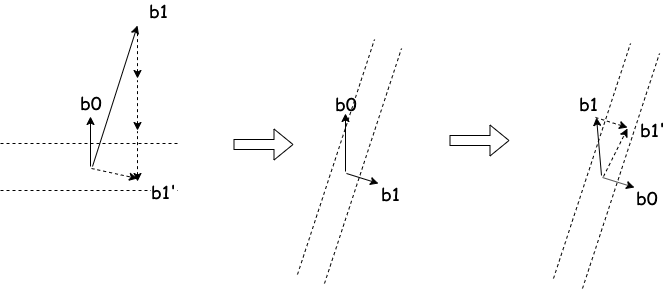
\includegraphics[width=0.8\textwidth]{files/BKZ-Lagrange.png}
\caption{Lagrange / Gauss Reduction}
\label{fig:bkz.lagrange}
\end{figure}

\subsubsection{Extension to Higher Dimensions}

The LLL algorithm is a generalization of the above procedure to multiple dimensions. However, due to the additional complexity and freedom of choices, this generalization can take many directions, and none of them is proved to be the optimal.

\paragraph{Lovasz condition.} A basis $\{\vb_0,\vb_1,\cdots,\}$ is said to satisfy the Lovasz condition for $\delta$ if for every $i$, $\|\vb_i\|/\|\vb_{i-1}\|\geq\delta-\mu_{i,i-1}^2$, where $\delta$ is a parameter s.t. $\delta\in(1/4,1)$. A typical choice of $\delta$ is $3/4$. Note that for the two-dimensional case, $\delta$ can take the value of $1$. However, for the general case, setting $\delta$ too close to $1$ costs efficiency.

\paragraph{LLL-reduced basis.} A basis $\{\vb_0,\vb_1,\cdots,\}$ is said to be LLL-reduced if it satisfies the Lovasz condition, and $\mu_{i,j}\leq 1/2$ for each pair of $i>j$.

\paragraph{LLL algorithm.} The LLL algorithm works as follows. Start with $i=1$, and for $j=i-1$ down to $0$, subtract $\lfloor\mu_{i,j}\rceil\vb_j$ from $\vb_i$, just as in the Lagrange/Gauss algorithm. After that, check if Lovasz condition holds for $\vb_i$ and $\vb_{i-1}$, and if so, increment $i$, and repeat the above process. If the Lovasz condition does not hold, swap $\vb_i$ and $\vb_{i-1}$ and decrement $i$, and repeat the above process.

Table \ref{tab:gen-lll} summarizes the ways LLL algorithm generalizes the Lagrange/Gauss algorithm.

\begin{table}[ht!]
\begin{tabular}{p{7cm}p{7cm}}
\hline
\textbf{In Lagrange/Gauss algorithm} & \textbf{In LLL algorithm} \\ \hline
Subtract $\lfloor\mu_{1,0}\rceil\vb_0$ from $\vb_1$ & Subtracting $\lfloor\mu_{i,j}\rceil\vb_j$ from $\vb_i$ for each $j$ from $i-1$ down to $0$ \\
Swap $\vb_0$ and $\vb_1$ if condition $\mu_{1,0}\leq1/2$ does not hold & Swap $\vb_{i-1}$ and $\vb_i$ if Lovasz condition does not hold, and decrement $i$ \\
Succeed when condition does hold & Increment $i$ if Lovasz condition does hold for $i$ \\ \hline
\end{tabular}
\caption{Generalization of LLL w.r.t. Lagrange/Gauss Algorithm}
\label{tab:gen-lll}
\end{table}

LLL runs in polynomial time, if $\delta\in(1/4,1)$, which is proved in the LLL paper \cite{lll1982factoring} as it is proposed in 1982.



\section{Basic BKZ Algorithm}
\label{sec:basic}

In this section, we introduce the most basic BKZ algorithm.
BKZ solves SVP by invoking LLL reduction and enumeration algorithms as subprocedures.

An execution of BKZ starts with input basis $(\vb_1,\cdots,\vb_n)$, and procedes in several rounds.
In each round, BKZ updates the basis by a procedure that is introduced as follows.
If in some round the basis stays unmodified after this procedure, the algorithm finishes.

In each round, BKZ iterates for $i$ from $1$ up to $n$.
In each iteration, BKZ first invokes the enumeration algorithm to find a solution of the exact SVP in the block $B_i$ of blocksize $\beta$, where $\beta$ is fixed as a global parameter for this algorithm.
Let $\vbs$ be the solution produced by the enumeration algorithm.
After that, $\vbs$ is inserted to the basis in the $i$'th position, and we get an extended basis $B'=(\vb_1,\vb_2,\cdots,\vb_{i-1},\vbs,\vb_i,\vb_{i+1},\cdots,\vb_n)$ of size $n+1$.
Finally, a reduction algorithm (LLL or small blocksize BKZ) is invoked to reduce $B'$ back into a basis of size $n$, which completes this one iteration.

Note that the vector $\vbs$ produced in each iteration is actually in the projective lattice by $\pi_i$.
Therefore, $\vbs$ is not necessarily a point in the original lattice.
However, it is easy to get the coefficients of $\vbs$ as a linear combination of the projected basis $(\pi_i(\vb_i),\cdots,\pi_i(\vb_{i+\beta-1}))$.
Apply the same linear combination to the original vectors $(\vb_i,\cdots,\vb_{i+\beta-1})$, and we get the original vector before projection.

Also note that in the start of each iteration, the basis is LLL-reduced, except in the first iteration in the first round.
Therefore, at the start of the BKZ algorithm, we apply the LLL reduction to the basis.

\section{BKZ 2.0}
\label{sec:bkz2}

The BKZ 2.0 algorithm proposed by Chen and Nguyen \cite{cn2011bkz} optimizes the original BKZ algorithm in the following ways:

\begin{itemize}
	\item \textbf{Extreme pruning technique:} Instead of applying the enumeration algorithm to the local block $B_i$, BKZ 2.0 chooses a low probability $p$, randomizes $B_i$ to $M=\lfloor 1/p\rceil$ blocks $G_1,\cdots,G_M$, and apply the enumeration algorithm to each $G_i$.
	\item \textbf{Limits point searching radius:} BKZ 2.0 sets the radius in the enumeration algorithm to $\min\{\alpha\GH(B_i),\|\vb_i^*\|\}$ where $\alpha=\sqrt{1.1}$.
	\item \textbf{Local-block preprocessing:} Before executing the enumeration algorithm, BKZ 2.0 applies a sequence of BKZ algorithms to preprocess the local block, to reduce the cost of enumeration algorithm.
	\item \textbf{Early termination:} BKZ 2.0 uses the early terminating technique \cite{hps2011analyzing}, by aborting BKZ with small number of rounds, instead of waiting for a round in which the basis stays unmodified.
\end{itemize}

\paragraph{BKZ 2.0 Simulator.} The paper \cite{cn2011bkz} that proposed BKZ 2.0 also presents a simulator to estimate the cost of BKZ 2.0 algorithm.
Based on the simulation results, \cite{cn2011bkz} also gives a table of cost of the enumeration algorithm $\Costbeta$ with respect to the blocksize $\beta$.

The simulator simulates the BKZ 2.0 algorithm by going through the procedure, without processing real vectors.
Instead, the simulator starts with the array $(\ell_1,\cdots,\ell_n)$ representing the lengths of Gram-Schmidt vectors $\|\vb_i^*\|$, and update the lengths in the rounds.

According to the table of simulation results, \cite{awht2016improved} extrapolates the cost as a function of $\beta$ as:

\begin{eqnarray}
\log_2(\Costbeta) = 0.000784314\beta^2 + 0.366078\beta - 6.125
\end{eqnarray}

Finally, the total cost of BKZ 2.0 (which is dominated by enumeration) is given by:

\begin{eqnarray}
\#rounds\cdot\sum_{i=1}^{n-1}\mathrm{Cost}_{\min\{\beta,n-i+1\}}
\end{eqnarray}


\section{Progressive BKZ}
\label{sec:pbkz}

Another strategy to improve BKZ algorithm is to progressively adapt the blocksize parameter during the execution of the algorithm.
The BKZ algorithms that make use of this strategy are called progressive BKZ algorithms.
The efficiency of BKZ is greatly impacted by the blocksize parameter.
Specifically, increasing the blocksize produces shorter vectors as solutions to the enumeration algorithm, with the drawback of increasing the computational cost.

The progressive strategy is based on the following observation: with fixed blocksize, the computational cost with gradually drop after each rounds.
Starting the BKZ with small blocksize, and gradually increasing it over the rounds of the execution, saves considerable amount of computation, without sacrificing the quality of the solution.

The progressive strategy is never implemented alone in the BKZ algorithm.
Instead, it is often used as one of the strategies in other works trying to improve the performance of the BKZ algorithm.
Therefore, there is no formal proposition of the so called ``The Progressive BKZ algorithm''.

The progressive strategy is usually utilized in two ways \cite{hr2019analyzing}:

\begin{enumerate}
\item \textbf{Globally}. The blocksize of the entire BKZ algorithm is updated gradually instead of being fixed.
\item \textbf{Locally}. The progressive strategy focuses on the local-block preprocessing, which could also be a BKZ algorithm.
\end{enumerate}

BKZ 2.0 belongs to the second category of progressive BKZ algorithms \cite{cn2011bkz}.
In fact, BKZ 2.0 implements the local-block preprocessing by another BKZ algorithm with much smaller blocksize, and makes use of the progressive strategy in this procedure.

One of the greatest challenges in the research of Progressive BKZ algorithm is to find an affective strategy to increase the blocksize.
This is also one of the key contribution of the algorithm proposed by \cite{awht2016improved}, which will be explained in detail in the next section.

\section{Improved Progressive BKZ}
\label{sec:ipbkz}

This section describes the improved progressive BKZ algorithm proposed by \cite{awht2016improved} in detail.
The most crucial of this algorithm is a strategy to decide when to increase the blocksize.
In summary, \cite{awht2016improved} implements a simulator which gives an estimation of the enumeration algorithm, provided with parameters $n$ and blocksize $\beta$.
At the end of each round, if the actual computational cost is less than the simulated cost, this is the time to increase the blocksize.
If the blocksize already reaches the predetermined $\beta_{end}$, the algorithm stops.

The improved progressive BKZ algorithm does not share many similarities with BKZ 2.0.
In fact, the only improvement they both have over the original BKZ is the preprocessing of local blocks.
However, the improved progressive BKZ makes use of the BKZ 2.0 simulator to compute the creteria for increasing blocksize.

\subsection{Optimizing parameters for local block}
\label{sub:opt}

The paper \cite{awht2016improved} proposes a method to obtain the optimal parameters $(\alpha,p)$ for the local block $B_i$ of size $\beta$ such that the efficiency of enumeration algorithm is optimized.

First, fix $\alpha$ and $\beta$, the optimal success probability $p$ and the resulting GSA constant $r$ can be obtained as follows:

\begin{eqnarray}
p &=& \frac{2}{\alpha^{\beta}} \label{eqn:alpha-p} \\
r &=& \left(\frac{\beta+1}{\alpha\beta}\right)^{4/(\beta-1)}\cdot V_{\beta}(1)^{4/(\beta(\beta-1))} \label{eqn:alpha-beta-r}
\end{eqnarray}

Conversely, by fixing $(\beta,r)$, one can first compute $\alpha$ by equation (\ref{eqn:alpha-beta-r}) and then get $p$ by equation (\ref{eqn:alpha-p}).
Therefore, for a given GSA constant $r$, it is possible to search the optimal $\beta$ which minimizes $\ENUMCost(B_i;\alpha,p)$.
An estimation of $\ENUMCost(B_i;\alpha,p)$ is given by:
\begin{eqnarray}
D = 2\alpha^{-\beta/2}\frac{V_{\beta/2}(1)V_{\beta}(1)^{-1/2}}{r^{\beta^2/16}} \label{eqn:enum-cost-alpha}
\end{eqnarray}
Then from equation (\ref{eqn:alpha-beta-r}) remove the $\alpha$ in \ref{eqn:enum-cost-alpha}:
\begin{eqnarray}
D\approx Const.\times r^{(\beta^2-2\beta)/16}\cdot\left(\frac{\beta}{e\pi}\right)^{\beta/4} \label{eqn:enum-cost}
\end{eqnarray}
Letting the partial derivative of $\beta$ be zero gives:
\begin{eqnarray}
\log(r)=\frac{\log (c_1\beta+c_2)}{c_3\beta+c_4}
\end{eqnarray}
where $c_1,c_2,c_3$ and $c_4$ are constants needed to be fitted.
Using the data collected from experiments, however, it is hard to fit the pairs $(\beta_i,\log r_i)$ with a single function $f(\beta)$.
Therefore, \cite{awht2016improved} ends up with two functions. In summary
\begin{eqnarray}
\log(r) = f(\beta)=\left\{\begin{matrix}f_1(\beta)&=&-18.2139/(\beta + 318.978) & \beta\leq 100 \\f_2(\beta)&=&(−1.06889/(\beta - 31.0345)) \cdot \log(0.417419\beta - 25.4889) & \beta > 100\end{matrix}\right. \label{eqn:f-beta}
\end{eqnarray}

With all the above equations, the $\ENUMCost(B_i;a,\alpha)$ is represented as a function of $\beta$.
To simplify this function, fitting experiments data pairs $(\beta,\ENUMCost(B_i;a,\alpha))$ gives:

\begin{eqnarray}
\log_2\MINCost(\beta):=\left\{\begin{matrix} 0.1375\beta + 7.153 & \beta\in[60,105] \\
0.000898\beta^2 + 0.270\beta - 16.97 & \beta>105 \end{matrix}\right.
\end{eqnarray}

Finally, for a fixed blocksize $\beta$, find the optimal parameters $(\alpha,p)$ by first computing $r$ with equation (\ref{eqn:f-beta}), then getting $\alpha$ by (\ref{eqn:alpha-beta-r}), and finally $p$ by (\ref{eqn:alpha-p}).

\subsection{Estimating Enumeration Cost}

The full enumeration cost (FEC) is the number of nodes in the searching-tree, which is given by
\begin{eqnarray}
\mathrm{FEC}(B)=\sum_{k=1}^n\frac{V_k(\GH(L))}{\prod_{i=n-k+1}^n\|\vb_i^*\|}
\end{eqnarray}
where $\|\vb_i^*\|$ is the Gram-Schmidt length.

To simulate the FEC, first simulate the Gram-Schmidt lengths $(\ell_1,\cdots,\ell_n)=\SimGSLengths(n,\beta)$ depending on dimension $n$ and blocksize $\beta$.
Then, simulate the Gaussian Heuristic by $\SimGH(\ell_1,\cdots,\ell_n)=V_n(1)^{-1/n}\prod_{j=1}^n\ell_j^{1/n}$.
We thus get the simulated FEC
\begin{eqnarray}
\SimFEC(\ell_1,\cdots,\ell_n)=\sum_{k=1}^n\frac{V_k(\SimGH(\ell_1,\cdots,\ell_n))}{\prod_{i=n-k+1}^n\ell_i}
\end{eqnarray}

\paragraph{Simulate Gram-Schmidt Lengths.}

First, set $\ell_n=1$, then compute $\ell_i$ backwards, by solving the following equation:
\begin{eqnarray}
\ell_i=\max\left\{\frac{\beta'}{\beta'+1}\alpha,\tau_{\beta'}\right\}\cdot\GH(\ell_i,\cdots,\ell_{i+\beta'-1}) \label{eqn:sim-gs}
\end{eqnarray}
where $\beta'=\min(\beta,n-i+1)$.

Next, we optimize the above GS-lengths for the last indexes $i>n-\beta+1$ as follows.
Select $(\alpha_i,p_i)$ for each $i$ such that $\SimENUMCost(\ell_i,\cdots,\ell_n;\alpha_i,p_i)=\MINCost(\beta)$, where $\alpha_i=(2/p_i)^{n-i+1}$ according to (\ref{eqn:alpha-p}).
Then solve (\ref{eqn:sim-gs}) again with $\alpha$ replaced by the previously selected $\alpha_i$.

The GS-lengths of the first $\beta$ indexes are also optimized.
However, it is not very clearly described in \cite{awht2016improved}.

% Finally, we optimize the GS-lengths for the first $\beta$ indexes.
% For a positive integer $b$, let $\beta_i=\beta+\max\{(b-i+1)/2,b-2(i-1)\}$ for $i=1$ to $b$.

\paragraph{Expected Number of BKZ Rounds for Specific Blocksize}

To estimate the number of rounds for a specific blocksize $\beta-1$, i.e. the number of rounds that are executed with this blocksize before the condition for increasing blocksize is satisfied, we simulate the execution of rounds by (a modified version of) the BKZ 2.0 simulator.
At the start, compute $(\ell_1,\cdots,\ell_n)$ by $\SimGSLengths(n,\beta-1)$.
Note that at this time $\SimFEC(\ell_1,\cdots,\ell_n)$ is equal to $\SimFEC(n,\beta-1)$ by definition.
Then update those lengths by the BKZ 2.0 simulator, until $\SimFEC(\ell_1,\cdots,\ell_n)$ drops below $\SimFEC(\beta,n)$.

Suppose at the end of round $t$, $\SimFEC(\ell_1,\cdots,\ell_n)$ is smaller than $\SimFEC(\beta,n)$, while before this round, $\SimFEC(\ell_1,\cdots,\ell_n)$ was larger.
Then the expected number of rounds is estimated to be somewhere between $t-1$ and $t$.
Specifically, assume the input of round $t$ is $(\ell_1',\cdots,\ell_n')$ and the output is $(\ell_1,\cdots,\ell_n)$, the ``somewhere'' is estimated to be $(t-1)+\frac{\SimFEC(\beta,n)-\SimFEC(\ell_1',\cdots,\ell_n')}{\SimFEC(\ell_1,\cdots,\ell_n)-\SimFEC(\ell_1',\cdots,\ell_n')}$.

\subsection{Optimizing Blocksize Strategy}

If the basis $B$ satisfies that $\mathrm{FEC}(B)<\SimFEC(n,\beta)$, then we say $B$ is $\beta$-reduced.
Currently, the blocksize strategy can be described as follows: at the start, $B$ is already $(\beta-1)$-reduced, the current blocksize is $\beta$, the BKZ rounds update the basis until at the end of some round $\mathrm{FEC}(B)<\SimFEC(n,\beta)$, i.e. $B$ is $\beta$-reduced, then update the blocksize to $\beta+1$.

This could be generalized by a blocksize strategy characterized by a tuple $(\beta^{start},\beta^{goal},\beta^{alg})$.
Concretely, at the start, $B$ is $\beta^{start}$-reduced, then update $B$ by blocksize $\beta^{alg}$, until $B$ is $\beta^{goal}$-reduced.
In this generalized definition, the original simple strategy can be described as the tuple $(\beta-1,\beta,\beta)$.
A complete blocksize strategy consists of a list of such tuples $\{(\beta_i^{start},\beta_i^{goal},\beta_i^{alg})\}_{i=1}^D$.
And a complete progressive BKZ algorithm loops through this list, apply the BKZ rounds with each strategy until $B$ is $\beta_i^{goal}$-reduced.

Usually, $\beta_i^{goal}$ is the same as $\beta_{i+1}^{start}$, so the list could be simplified to $\{(\beta_i^{goal},\beta_i^{alg})\}_{i=1}^D$.
Notice that $\beta_1^{start}$ is not defined in this way, which we simply neglect, because at the start of the BKZ algorithm $B$ is only LLL-reduced, and it is not sure if $B$ is $\beta$-reduced for any $\beta$.

Let $\TimeBKZ(n,\beta_{i-1}^{goal}\xrightarrow{\beta_i^{alg}}\beta_i^{goal})$ denote the time required for the BKZ rounds to update a $\beta_{i-1}^{goal}$ reduced basis to one that is $\beta_i^{goal}$-reduced with blocksize $\beta_i^{alg}$.
The goal of optimizing blocksize strategy is to minimize the total time:
\begin{eqnarray}
\sum_{i=1}^D\TimeBKZ(n,\beta_{i-1}^{goal}\xrightarrow{\beta_i^{alg}}\beta_i^{goal})
\end{eqnarray}
Denote by $\TimeBKZ(n,\beta^{goal})$ the minimized total time of the entire BKZ algorithm, whose input is a basis that is LLL-reduced, and the output is one that is $\beta^{goal}$-reduced.
The minimization is taken over all possible block strategies that are ended with $\beta^{goal}$.

By definition, we can also write $\TimeBKZ(n,\beta^{goal})$ recursively as follows:
\begin{eqnarray}
\TimeBKZ(n,\beta^{goal})=\min_{\beta',\beta^{goal}}\left\{\TimeBKZ(n,\beta')+\TimeBKZ(n,\beta'\xrightarrow{\beta^{alg}}\beta^{goal})\right\} \label{eqn:timebkz}
\end{eqnarray}
In this way, we can compute $\TimeBKZ(n,\beta^{goal})$ in the dynamic programming way by first computing $\TimeBKZ(n,\beta')$ for all $\beta'<\beta^{goal}$, then minimizing equation (\ref{eqn:timebkz}) over all pairs of $(\beta',\beta^{alg})$.

\subsection{Implementation of BKZ Rounds and Computational Cost}

Now is the time to actually compute the $\TimeBKZ(n,\beta^{start}\xrightarrow{\beta^{alg}}\beta^{goal})$.
By definition
\begin{eqnarray}
&&\TimeBKZ(n,\beta^{start}\xrightarrow{\beta^{alg}}\beta^{goal})=\nonumber\\
&&\sum_{t=1}^{\#rounds}\sum_{i=1}^{n-1}\left[\text{Time of processing local block $B_i$ with parameter $(\alpha,p)$}\right]
\end{eqnarray}
where $\alpha$ and $p$ are selected according to the strategy described in Section \ref{sub:opt} with blocksize $\beta_{alg}$.

One iteration in the BKZ round in the improved progressive BKZ algorithm can be decomposed into the following steps.
We will give the cost estimation for each step as we describe them.

\paragraph{Compute Gram-Schmidt lengths.}
In this step, we need to compute the Gram-Schmidt variables $\|\vb_i^*\|$ and $\mu_{ij}$ for the local block $B_i$. They are needed in the computation in the following steps, for example, to estimate the optimal parameters $\alpha$ and $p$.
In implementation, the Gram-Schmidt variables could be precomputed for the entire basis $B$, and for each block $B_i$ we can simply copy the corresponding parts.

The cost of this step is negligible.

\paragraph{Compute bounding coefficients.}
We compute the bounding coefficients $(R_1,\cdots,R_{\beta})$ using Aono's precomputing technique.
Recall that these bounding coefficients are used in the enumeration algorithm for each layer in the searching tree.

The cost of this step is negligible.

\paragraph{Preprocess local block.}
We preprocess the local block $B_i$ using this improved progressive BKZ algorithm, but with much smaller blocksizes.
The blocksize strategy here takes the simple one-by-one strategy starting from $15$.

The cost of this step is estimated to be that of the enuemration times a constant $A_{Preprocess}$.
The constant will be determined by experiments.

\paragraph{Optimize bounding coefficients.}
We optimize the bounding coefficients $(R_1,\cdots,R_{\beta})$ after preprocessing $B_i$, if the estimated number of nodes in the searching tree is larger than $10^8$.
This procedure is a simple algorithm that considers random perturbation of $(R_1,\cdots,R_{\beta})$, which is also used in BKZ 2.0.

The cost of this optimization step is significantly smaller than the enumeration step.
In small blocksizes, the optimization is often skipped, and the time consumption of this step is approximately zero.
For large blocksizes, the enumeration step is also much larger than this step.
Therefore, it is safe to ignore the computational cost here.

\paragraph{Enumeration.}
The enumeration is implemented in the standard way.
In the end, it outputs $h=16$ vectors whose projective lengths are small, and store them in $(\vv_1,\cdots,\vv_h)$.

The cost of this step is given by $A_{Enum}\cdot\beta\cdot\SimENUMCost(\ell_i,\cdots,\ell_{i+\beta-1};\alpha,p)$, where $A_{Enum}$ is a constant.

\paragraph{Construct degenerated basis.}
After we get the vectors $(\vv_1,\cdots,\vv_h)$ from enumeration, we select some of them and insert into the $i$'th position of basis $(\vb_1,\cdots,\vb_n)$ as follows.
Starts with $\hat{B}=(\vb_1,\cdots,\vb_{i-1})$.
In each step we select and remove one $\vv_j$ from the vectors, and append it to the end of $\hat{B}$.
The $\vv_j$ selected in each step is the one that minimizes the norm of the projection of $\vv_j$ onto the current $\hat{B}$, which is denoted by $\|\pi'(\vv_j)\|$.
Moreover, it is required that $0<\|\pi'(\vv_j)\|<\|\text{last vector of } \hat{B}\|$.
If no such $\vv_j$ satisfies this requirement, then stop the procedure and return the current $\hat{B}$ joined with the rest of basis, i.e. $(\vb_i,\cdots,\vb_n)$.

This cost of this step is negligible.

\paragraph{Apply LLL to degenerated basis.}
Assume that the degenerated basis created in the previous step is larger than the blocksize by $g$, i.e. the size is $i+\beta'-1+g$.
We can assume that the first $i-1$ vectors in the basis is already LLL-reduced, the computational cost can be approximated by applying LLL to the later $\beta'+g$ vectors in the basis, which is $O(n^2\cdot\beta^2)=A_1\cdot\beta^2 n^2$ where $A_1$ is constant.

\paragraph{Total Cost and Constants Fitting.}
Finally, the time cost for the entire BKZ algorithm can be expressed as follows.
\begin{eqnarray}
\mathrm{Time}(n,\beta,A_1,W_1)=\sum_{\beta^{start}}^{\beta^{goal}}\sum_{t=1}^{\#rounds}
\left[A_1\cdot\beta^2 n^3+W_1\cdot\beta\sum_{i=1}^{n-1}\ENUMCost(B_i;\alpha,p)\right]
\end{eqnarray}
where $A_1$ and $W_1$ are constants that are determined by experiments.
The coefficients are fitted by standard curve fitting method in semi-log scale.
The results given in \cite{awht2016improved} are $A_1=1.5\cdot 10^{-10}$ and $W_1=1.5\cdot 10^{-8}$.


\subsection{Pre/Post-Processing the Basis}

By preprocessing or postprocessing the basis, it is possible to enhance the speed of the progressive BKZ algorithm.
The preprocessing works similar to the extreme pruning algorithm proposed by \cite{gnr2010lattice}, by generating a number of randomized bases, reducing each of them by this progressive BKZ algorithm.
In the postprocessing part, apply the enumeration algorithm with low success probability to each of the basis to find short vectors.

Concretely, the algorithm works as follows.
Randomly generate $M$ unimodular matrices $U_i$, and produces $M$ randomized basis $U_iB$.
Then apply the progressive BKZ to each of the random basis.
In the postprocessing, set $\alpha=\gamma$ and probability $p=2\cdot\gamma^{-n}/M$ and apply the enumeration algorithm.


\section{Conclusion}
\label{sec:con}

In this article we introduced the series of BKZ algorithms, including the preliminaries necessary for understanding BKZ.
Specifically, we introduced Gram-Schmidt reduction, Gaussian Heuristic, LLL reduction and the enumeration algorithm.
Based on the knowledge of above, we described the details of the basic BKZ algorithm, BKZ 2.0, Progressive BKZ, and finally the improved progressive BKZ proposed by \cite{awht2016improved}.

The improved progressive BKZ modifies the original BKZ algorithm in the following aspects:
\begin{enumerate}
	\item Implement the progressive strategy by increasing the blocksize when the actual cost of a round is smaller than the simulated cost.
	\item Terminate the algorithm when the blocksize increases over $\beta_{end}$.
	\item Preprocess the local block with progressive BKZ algorithm of smaller blocksize.
	\item Apply extreme pruning technique globally.
\end{enumerate}

\bibliographystyle{alpha}
\bibliography{reference}

\end{document}